\documentclass{article}
\usepackage[utf8]{inputenc}
\usepackage[spanish]{babel}
\usepackage{amssymb}
\usepackage{amsmath}

% Formato de página
\usepackage[letterpaper, margin = 1.5cm]{geometry}

% Más opciones para enumerar
\usepackage{enumitem}

% Manejo de imágenes
\usepackage{graphicx}
\usepackage{wrapfig}
\graphicspath{{img/}}
\usepackage{float}

\begin{document}
    \title{
        Fundamentos de bases de datos \\
        Tarea 5 \\
        Lenguaje de consulta SQL
    }
    \author{
        Díaz Gómez Silvia \\
        Eugenio Aceves Narciso Isaac \\
        Quiroz Castañeda Edgar
    }
    \date {
        13 de Mayo del 2019    
    }
    \maketitle
    Se tiene el siguiente esquema de bases de datos acerca de médicos, pacientes, ingresos consultas y
    especialidades:\\
    
   \begin{center}
   	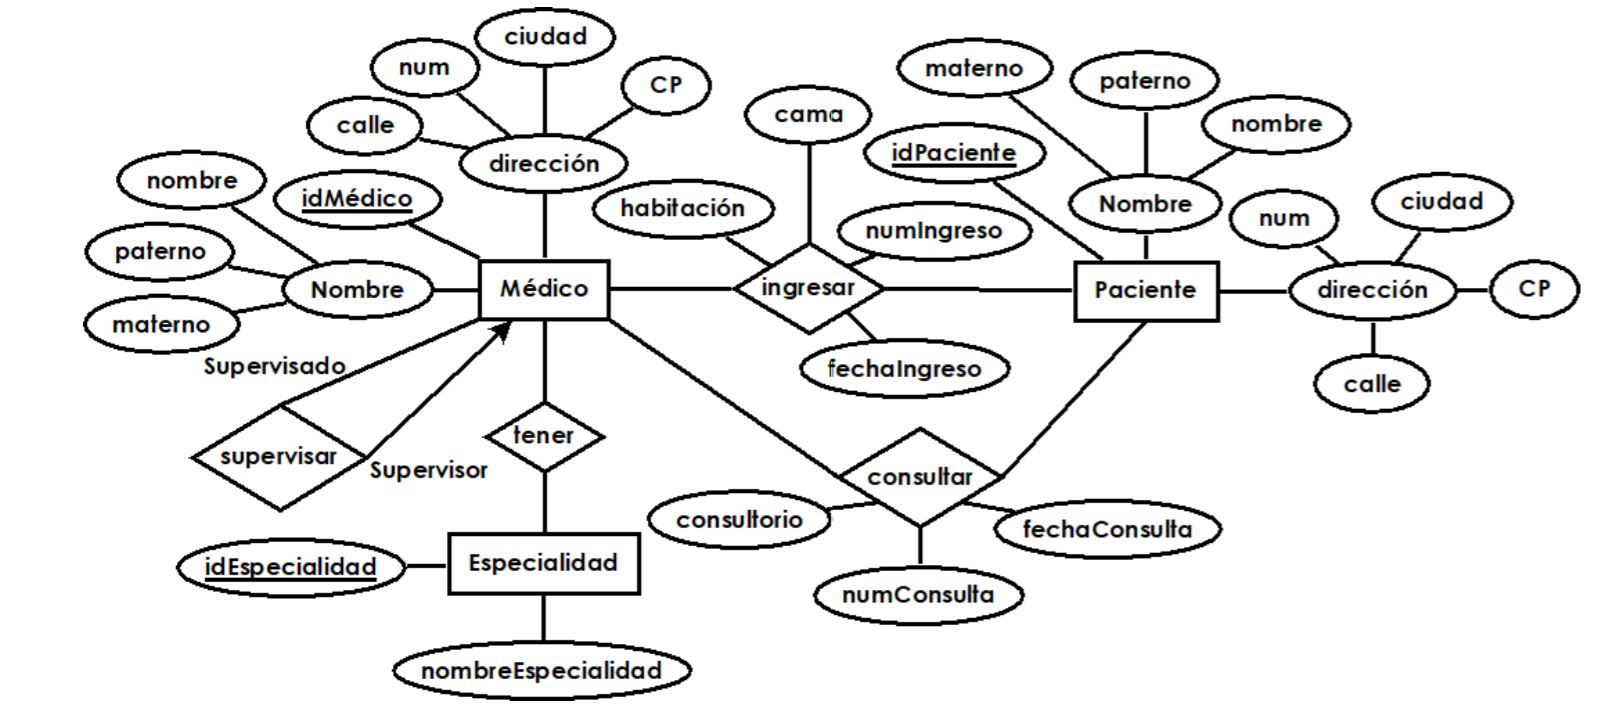
\includegraphics[width=1\textwidth]{img.JPG}
   \end{center}
    
    Resuelve los siguientes puntos:
    \begin{enumerate}
    	\item Traduce el modelo E-R a su correspondiente modelo relacional, indicando claramente las llaves
    	primarias y foráneas. No incluyas relaciones redundantes.\\
    	
    	\begin{center}
    		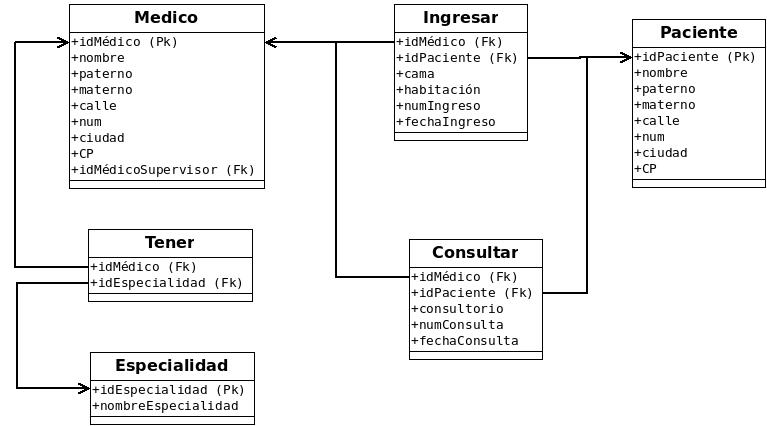
\includegraphics[width=1\textwidth]{DiagramaRelacional.jpeg}
    	\end{center}
   \end{enumerate}
\end{document}   	